\documentclass[../../main.tex]{subfiles}
\begin{document}

{\bf[解]}

$D,E$の領域は
\begin{align}
  \begin{cases}
    D: x^2 \le y \\
    E: (x-4)^2 \le y
  \end{cases} \label{eq:1}
\end{align}
である．$D$と$E$のグラフは下図のようになる．

\begin{figure}[htb]
  \centering
  \begin{tikzpicture}[scale=1.0, >=stealth, every node/.style={font=\small}]
    \begin{scope}
      \clip (-0.5,0) rectangle (5,4.6);
      \fill[pattern=north east lines, pattern color=black!50]
      plot[domain=-0.5:5, samples=80] (\x,{\x*\x}) -- (5,10) -- (-0.5,10) -- cycle;
      \fill[pattern=north east lines, pattern color=black!50]
      plot[domain=-0.5:5, samples=80] (\x,{(\x-4)*(\x-4)}) -- (5,10) -- (-0.5,10) -- cycle;
    \end{scope}

    \draw[->] (-0.5,0) -- (5,0) node[right] {$x$};
    \draw[->] (0,-0.3) -- (0,4.6) node[above] {$y$};
    \node[below left=1pt] at (0,0) {$O$};

    \draw[thick] plot[domain=-0.5:2.9, samples=60] (\x,{\x*\x}) node[above right=1pt] {$y=x^2\,(D)$};
    \draw[thick] plot[domain=1.1:4.5, samples=60] (\x,{(\x-4)*(\x-4)});
    \node[right=1pt] at (3.9,1.3) {$y=(x-4)^2\,(E)$};

    \draw[dotted] (2,0) -- (2,4) -- (0,4);
    \node[below=1pt] at (2,0) {$2$};
    \node[left=1pt] at (0,4) {$4$};
    \node[below=1pt] at (4,0) {$4$};
  \end{tikzpicture}
  \caption{領域 $D:x^2\le y$（斜線）と $E:(x-4)^2\le y$（斜線）}
\end{figure}

ついで $U$ の領域について考える．
$y=x^2$を$P(a,b)$に関して対称移動すると，
\begin{align}
  2b-y = (2a-x)^2 \label{eq:2}
\end{align}
にうつるから，
\begin{align}
  U:y\le -(x-2a)^2+2b \quad (\equiv f(x)) \label{eq:3}
\end{align}
となる．

さて，簡単のため題意の条件を
\begin{align}
  A&:D\cap U\not=\emptyset \\
  B&:E\cap U\not=\emptyset \\
  C&:D\cap E\cap U=\emptyset
\end{align}
とおく．
まず$A\cap B$が成り立たないといけないから $D,U$ および$ E, U$ が共有点を持つ．
さらに$C$から$3$つの曲線全ての共有点は存在しない．よって題意の$(*)$の条件は
\begin{itemize}
  \item $y=f(x)$と$y=x^2$が$x<2$に共有点を持つ． \\
  \item $y=f(x)$と$y=(x-4)^2$が$2<x$に共有点を持つ．
\end{itemize}
すなわち
\begin{itemize}
  \item $f(x)=x^2$ が$x<2$のみに実解を持つ．\\
  \item $f(x)=(x-4)^2$が$2<x$のみに実解を持つ．
\end{itemize}
である．

\begin{figure}[htb]
  \centering
  \begin{tikzpicture}[scale=1.0, >=stealth, every node/.style={font=\small}]
    \begin{scope}
      \clip (-0.5,0) rectangle (5,4.6);
      \fill[gray!25]
      plot[domain=-0.5:5, samples=80] (\x,{-(\x-2)*(\x-2)+3}) -- (5,-10) -- (-0.5,-10) -- cycle;
      \fill[pattern=north east lines, pattern color=black!50]
      plot[domain=-0.5:5, samples=80] (\x,{\x*\x}) -- (5,10) -- (-0.5,10) -- cycle;
      \fill[pattern=north east lines, pattern color=black!50]
      plot[domain=-0.5:5, samples=80] (\x,{(\x-4)*(\x-4)}) -- (5,10) -- (-0.5,10) -- cycle;
    \end{scope}

    \draw[->] (-0.5,0) -- (5,0) node[right] {$x$};
    \draw[->] (0,-0.3) -- (0,4.6) node[above] {$y$};
    \node[below left=1pt] at (0,0) {$O$};

    \draw[thick] plot[domain=-0.5:2.9, samples=60] (\x,{\x*\x}) node[above right=1pt] {$y=x^2\,(D)$};
    \draw[thick] plot[domain=1.1:4.5, samples=60] (\x,{(\x-4)*(\x-4)});
    \node[right=1pt] at (3.9,1.3) {$y=(x-4)^2\,(E)$};
    \draw[thick, dashed] plot[domain=0.2:3.8, samples=60] (\x,{-(\x-2)*(\x-2)+3});
    \node[above=6pt] at (2,3) {$y=f(x)\,(U)$};

    \draw[dotted] (2,0) -- (2,4.6);
    \node[below=1pt] at (2,0) {$2$};

    % U と D の交点（x<2）
    \fill (0.293,0.0858) circle (1pt);
    \fill (1.707,2.914) circle (1pt);
    % U と E の交点（2<x）
    \fill (2.293,2.914) circle (1pt);
    \fill (3.707,0.0858) circle (1pt);
  \end{tikzpicture}
  \caption{$D,E,U$ の位置関係（代表例 $a=1,b=\dfrac{3}{2}$）．$D,E$ は斜線，$U$ は灰色で示す．$U$ の境界 $y=f(x)$ は $D$ と $x<2$ で，$E$ と $2<x$ でのみ交わる}
\end{figure}

\subparagraph{$f(x)=x^2$ が$x<2$のみに実解を持つ}

\begin{figure}[htb]
  \centering
  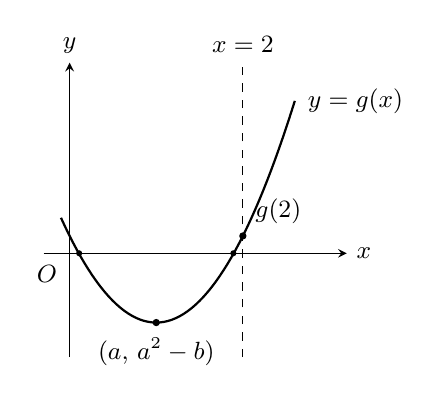
\begin{tikzpicture}[scale=1.1, >=stealth, every node/.style={font=\small}]
    \draw[->] (-0.3,0) -- (3.2,0) node[right] {$x$};
    \draw[->] (0,-1.2) -- (0,2.2) node[above] {$y$};
    \node[below left=1pt] at (0,0) {$O$};

    \draw[thick] plot[domain=-0.1:2.6, samples=60] ({\x}, {(\x-1)*(\x-1)-0.8}) node[right=1pt] {$y=g(x)$};
    \draw[dashed] (2,-1.2) -- (2,2.2) node[above] {$x=2$};

    \fill (1,-0.8) circle (1.2pt) node[below=2pt] {$(a,\,a^2-b)$};
    \fill (2,0.2) circle (1.2pt) node[above right=1pt] {$g(2)$};
    \fill (0.11,0) circle (1pt);
    \fill (1.89,0) circle (1pt);
  \end{tikzpicture}
  \caption{$y=g(x)$ の概形（代表例）．頂点の $x$ 座標 $a<2$ かつ $g(2)>0$ のとき，$2$ 解はともに $x<2$ の範囲にある}
\end{figure}

$f(x)=x^2$を整理して
\begin{align}
  g(x) \equiv (x-a)^2+a^2-b=0
\end{align}
の左辺$g(x)$とおき，判別式を$D_1$とおく．
$g(x)=0$が$x<2$にのみ実解をもつ条件は，
\begin{align}
  &
  \begin{cases}
    D_1/4\ge0 \\
    \text{軸}: a<2 \\
    \text{端}: g(2)>0
  \end{cases}\\
  \iff
  &
  \begin{cases}
    (2a)^2-2(4a^2-2b)\ge 0 \\
    a<2 \\
    2a^2-4a+4-b>0
  \end{cases}\\
  \iff
  &
  \begin{cases}
    b\ge a^2 \\
    a<2 \\
    b<2(a-1)^2+2 \\
  \end{cases} \label{eq:4}
\end{align}
である．

\subparagraph{$f(x)=(x-4)^2$が$2<x$のみに実解を持つ}

\begin{figure}[htb]
  \centering
  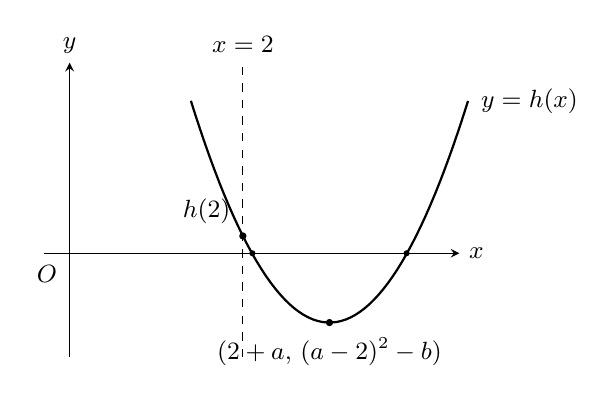
\begin{tikzpicture}[scale=1.1, >=stealth, every node/.style={font=\small}]
    \draw[->] (-0.3,0) -- (4.5,0) node[right] {$x$};
    \draw[->] (0,-1.2) -- (0,2.2) node[above] {$y$};
    \node[below left=1pt] at (0,0) {$O$};

    \draw[thick] plot[domain=1.4:4.6, samples=60] ({\x}, {(\x-3)*(\x-3)-0.8}) node[right=1pt] {$y=h(x)$};
    \draw[dashed] (2,-1.2) -- (2,2.2) node[above] {$x=2$};

    \fill (3,-0.8) circle (1.2pt) node[below=2pt] {$(2+a,\,(a-2)^2-b)$};
    \fill (2,0.2) circle (1.2pt) node[above left=1pt] {$h(2)$};
    \fill (2.11,0) circle (1pt);
    \fill (3.89,0) circle (1pt);
  \end{tikzpicture}
  \caption{$y=h(x)$ の概形（代表例）．頂点の $x$ 座標 $2+a>2$ かつ $h(2)>0$ のとき，$2$ 解はともに $2<x$ の範囲にある}
\end{figure}

$f(x)=(x-4)^2$を整理して
\begin{align}
  h(x) \equiv \left\{x-(2+a)\right\}^2+(a-2)^2-b=0
\end{align}
の左辺$h(x)$とおき，判別式を$D_2$とおく．
$h(x)=0$が$2<x$にのみ実解をもつ条件は，
\begin{align}
  &
  \begin{cases}
    D_2/4 \ge 0 \\
    \text{軸}: 2 < a+2 \\
    \text{端}: h(2) > 0
  \end{cases}\\
  \iff
  &
  \begin{cases}
    (a-2)^2-b \le 0 \\
    0 < a \\
    a^2 + (a-2)^2 -b > 0
  \end{cases} \\
  \iff
  &
  \begin{cases}
    (a-2)^2 \le b \\
    0<a \\
    2(a-1)^2+2>b
  \end{cases} \label{eq:5}
\end{align}
である．
\casesend

以上をまとめて\cref{eq:4}かつ\cref{eq:5}が求める条件で，
図示すると下図斜線部である．境界は実線のみ含む．

よって領域は以下の通りである．$\cdots$(答)
\begin{align}
  \begin{cases}
    a^2 \le b < 2(a-1)^2 + 2 \\
    (a-2)^2 \le b < 2(a-1)^2 + 2 \\
    0<a<2
  \end{cases}
\end{align}

\begin{figure}[htb]
  \centering
  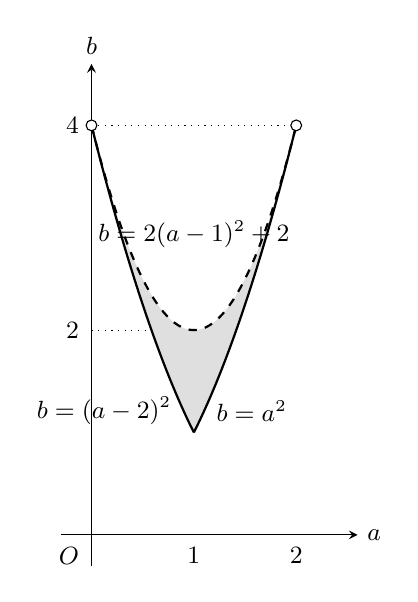
\begin{tikzpicture}[scale=1.3, >=stealth, every node/.style={font=\small}]
    \draw[->] (-0.3,0) -- (2.6,0) node[right] {$a$};
    \draw[->] (0,-0.3) -- (0,4.6) node[above] {$b$};
    \node[below left=1pt] at (0,0) {$O$};

    \draw[dotted] (0,4) -- (2,4);
    \draw[dotted] (0,2) -- (1,2);
    \node[left=1pt] at (0,4) {$4$};
    \node[left=1pt] at (0,2) {$2$};
    \node[below=1pt] at (2,0) {$2$};
    \node[below=1pt] at (1,0) {$1$};

    \fill[gray!25] plot[domain=0:1, samples=40] (\x,{(\x-2)*(\x-2)})
    -- plot[domain=1:2, samples=40] (\x,{\x*\x})
    -- plot[domain=2:0, samples=60] (\x,{2*(\x-1)*(\x-1)+2})
    -- cycle;

    \draw[dashed, thick] plot[domain=0:2, samples=60] (\x, {2*(\x-1)*(\x-1)+2});
    \node[above=4pt] at (1,2.6) {$b=2(a-1)^2+2$};

    \draw[thick] plot[domain=0:1, samples=40] (\x, {(\x-2)*(\x-2)});
    \draw[thick] plot[domain=1:2, samples=40] (\x, {\x*\x});
    \node[left=1pt] at (0.9,{(0.9-2)*(0.9-2)}) {$b=(a-2)^2$};
    \node[right=1pt] at (1.1,{1.1*1.1}) {$b=a^2$};

    \draw[fill=white] (0,4) circle (1.5pt);
    \draw[fill=white] (2,4) circle (1.5pt);
  \end{tikzpicture}
  \caption{$(a,b)$ 平面における求める領域（灰色部）．下側境界（実線）は含み，上側境界 $b=2(a-1)^2+2$（破線）と両端点 $(0,4),(2,4)$ は含まない}
\end{figure}

\newpage
\end{document}
